\section{Introduction}\label{paper:olguinmunoz2019edgedroid:sec:intro}

There is increasing interest from academia and industry in novel applications such as immersive \gls{AR} or \gls{WCA}~\cite{chatzopoulos2017hyperion,ha2014towards}, also known as human-in-the-loop applications.
These applications aim to seamlessly integrate into the lives of users to provide real-time, context-aware information by capturing user and environment information and leveraging compute-intensive algorithms to analyze the data in order to provide real-time feedback to the user.
Sensory input, such as video, audio, and other user-related data such as orientation and movement, are examples of what is typically captured, while the backend generally employs machine learning technologies such as \glspl{DNN}~\cite{ha2014towards}.
\Cref{paper:olguinmunoz2019edgedroid:fig:pipeline2} depicts such a system.
These applications are highly latency sensitive, measuring latency as the time from the capture of the sensory information until feedback is received.
Delays above a certain threshold can hurt the user experience or even make the application unusable~\cite{chen2017empirical}.

In literature, these challenging latency requirements have so far mainly been addressed through research on the optimal placement of the compute process.
There is a broad understanding today that with the advent of edge computing, human-in-the-loop applications will become viable~\cite{bittmann2017edge,flinn2012cyber,chen2017empirical,ha2013just}.
However, with respect to end-to-end latency, there are many more trade-offs involved than merely the question of where the compute backend is placed.
A human-in-the-loop application consists of various processing steps that can be influenced during the development of the application.
What kind of compression to apply to the sensory input on the uplink; which backend algorithms to utilize; how to stage the backend; when to send feedback to the human users; and how to manage congestion on the loop, as well as wireless channel fluctuations --- all these design choices impact the latency of the application.
There are also many design choices in the infrastructure: how is the sensory input conveyed to the point of computation (i.e.\ by which wireless system; with which transmission/prioritization scheme); which hardware is running at the backend; which operating system; how is the feedback conveyed back to the human user?
Finally, in production use these applications will most likely run concurrently with others.
How does this, together with other best-effort applications, impact the latencies perceived by the human user?
Existing studies~\cite{ha2014towards,chen2015early,satyanarayanan2009case,chatzopoulos2017hyperion} of this class of applications have only lightly touched upon these issues~\cite{chen2017empirical}.
On the other hand, recently published models for end-to-end latency of edge computing architectures~\cite{al_zubaidy2015performance,schiessl2017finite} are quite complex, while not accounting for the specifics of human-in-the-loop applications.
We only have a coarse understanding of the many degrees of freedom upon which end-to-end latency depends.

The goal of this paper is to provide a methodological approach to studying these latency trade-offs, along with a tool, EdgeDroid 1.0\footnote{We plan to make the EdgeDroid 1.0 benchmarking suite available as Free and Open Source Software and the recorded traces under a Creative Commons License.}, that simplifies the benchmarking of human-in-the-loop applications.
We view EdgeDroid 1.0 to be the very first, and simplest, of a family of tools that will embody increasingly sophisticated and accurate models of user behavior.

Due to the complex nature of the applications and the infrastructure, we opt for experimentally studying the trade-offs in a repeatable and controllable fashion.
This is difficult mainly due to the unpredictable reaction of human users to the feedback from the backend --- a user might very well misinterpret the feedback handed to them.
EdgeDroid 1.0 mimics the operation of human-in-the-loop applications by replaying recorded traces of sensory input.
This sensory information is then processed by the original compute process at the backend, generating feedback.
However, this feedback is not processed by humans, but by a parameterizable model of human reaction.
Through synchronized time tracking at the different processing points of the application, EdgeDroid 1.0 allows for accurate measurements of key performance metrics such as the distribution of delays across the application pipeline.
Analysis of these metrics can be performed down to the individual input sample, allowing us to zoom into the internal model of the application under consideration.
Thus, EdgeDroid 1.0 allows us to illuminate the many latency trade-offs existing at the level of the infrastructure, as well as the level of the application.
It can also be used for debugging and validation, by comparing the expected execution flow of a particular trace with the actual flow during the benchmarking.
To the best of our knowledge, this experimentally-driven benchmarking approach is the first one towards experimental performance characterization and potential optimization of human-in-the-loop applications

The rest of the paper is structured as follows:
\cref{paper:olguinmunoz2019edgedroid:sec:background} presents some background on human-in-the-loop applications.
\cref{paper:olguinmunoz2019edgedroid:sec:approach} discusses the general approach taken with EdgeDroid, while \cref{paper:olguinmunoz2019edgedroid:sec:implementation} exposes the implementation details for EdgeDroid 1.0.
We show the value of the tool through use case analysis in \Cref{paper:olguinmunoz2019edgedroid:sec:usecases,paper:olguinmunoz2019edgedroid:sec:results}, before discussing future work and concluding in \cref{paper:olguinmunoz2019edgedroid:sec:conclusions}.


%\section{Design \& Implementation}\label{sec:design_impl}
\section{Background}\label{paper:olguinmunoz2019edgedroid:sec:background}

Human-in-the-loop applications are novel applications aiming to seamlessly integrate into the lives of users and provide real-time, context-aware information.

Given the wide range of applications which fall under this concept, we have chosen to focus our initial efforts on one particular category: task-guidance \gls{WCA}~\cite{ha2014towards}.
We have chosen this type of application for two reasons: one, their relative simplicity in terms of execution flow, and two, the already well-established existing body of work~\cite{ha2014towards,chen2015early,chen2017empirical}.
Task-guidance \gls{WCA} applications aim to guide users in the execution of a task by monitoring user actions and providing real-time instructions, usually through wearable sensors and gadgets such as the Google Glass platform.
They have many potential use cases including training and assistance for professionals performing complex tasks.
Imagine for instance a specialized technician performing field repairs on a complex piece of machinery.
A task-guidance \gls{WCA} application could offer real-time guidance in this task, by analyzing a real-time video feed from the technician's head-mounted camera and providing step-by-step repair instructions.

Broadly speaking, task-guidance \gls{WCA} applications (and human-in-the-loop in general) process a multitude of inputs in parallel, which are also usually continuous, multidimensional and time-sensitive, e.g.\ video and audio feeds.
These inputs are passed to the computation backend, where they are processed in the pipeline depicted in \cref{paper:olguinmunoz2019edgedroid:fig:pipeline2}.
The first step of the backend processing is detection, which acts as a filter for irrelevant inputs.
For example, this step could consist of a computer vision detector which discards all frames for which the relevant features were not detected or which were below a set threshold.
%Given the often complex nature of the inputs, this stage usually employs Machine Learning to process them.
The remaining inputs pass on to the symbolic representation stage, where features are extracted and parameterized for subsequent computation.
For video frames, this parametrization would usually convert the visual data into a matrix representation of the  relevant features.
This representation of the inputs then continues on to the task model, where the actual application logic resides, before finally passing through the feedback generation stage at which point human-parseable feedback is generated; for instance, animations and voice commands.

\begin{figure}[b]
    \centering
    \adjustbox{scale=0.65}{
        \ttfamily\centering%\fbox{%
        \begin{tikzpicture}[align=center,
                        node distance=0.7cm and 0.7cm,
                        every initial by arrow/.style={draw=none, minimum size=0em},
                        %node styles:
                        block_center/.style ={rectangle, draw=black, thick, fill=white,
                                        text width=8em, text centered, minimum height=4em},
                        block_left/.style ={rectangle, draw=black, thick, fill=white,
                                        text width=16em, text ragged, minimum height=4em, inner sep=6pt},
                        block_noborder/.style ={rectangle, draw=none, thick, fill=none,
                                        text width=18em, text centered, minimum height=1em},
                        block_assign/.style ={rectangle, draw=black, thick, fill=white,
                                        text width=18em, text ragged, minimum height=3em, inner sep=6pt},
                        block_lost/.style ={rectangle, draw=black, thick, fill=white,
                                        text width=16em, text ragged, minimum height=3em, inner sep=6pt},
                        block_rounded/.style ={rectangle, draw=black, thick, fill=white,
                                        text width=8em, text centered, rounded corners=.55cm, minimum height=4em},
                        line/.style ={draw, thick, -{Latex[length=3mm]}, shorten >=0pt}
                ]

                \matrix [column sep=5mm,row sep=3mm] (top) {
                        \node [block_center] (detect) {Detection};
                         & \node [block_center] (repr) {Symbolic\\Repr.};
                         & \node [block_center] (model) {Task Model\\$M\{S, E\}$};
                         & \node [block_center] (feedback) {Feedback\\Generation}; \\[3ex]
                };

                \matrix [column sep=13mm,row sep=3mm, below=of top] (bottom) {
                        \node [block_rounded] (sensors) {On-body\\Sensors};
                         %& \node [block_rounded] (user) {Human User};
                         %&\node[cloud, draw, black, text centered, cloud ignores aspect=false] (user) {Human User};
                         & \node[maninblack, minimum height=5em] (user) {\Large Human User};
                         & \node [block_rounded] (hud) {HUD, Speakers,\\etc.}; \\
                };

                %\Smiley[1, below of=bottom] (smiley);


                \begin{scope}[every path/.style=line]
                        \path (detect) -- (repr);
                        \path (repr) -- (model);
                        \path (model) -- (feedback);
                        \path (feedback) -- (hud);
                        \path (hud) -- (user);
                        \path (user) -- (sensors);
                        \path (sensors) -- (detect);
                \end{scope}

                % % Place nodes       
                % \node [initial, state, draw=none, initial text=, minimum size=0em] (input) {};
                % \node [state, right=1cmof input, minimum size=7em] (detect) {Detection};
                % \node [state, right=2cm of detect, minimum size=7em] (symb) {Symbolic\\Repr.};
                % \node [state, right=.5cm of symb, minimum size=7em] (feedback) {Feedback\\Gen.};
                % \node [state, accepting, draw=none, right=1cm of feedback, minimum size=0em] (output1) {};
                % \node [state, accepting, draw=none, below=1.4cm of output1, minimum size=0em] (output2) {};

                % % Draw edges
                % \path[draw, -{Latex[length=3mm]}]
                % (input) edge node[above left] {Input} (detect)
                % (detect) edge node[above] {LEGO bricks\\in input} (symb)
                % (symb) edge node {} (feedback)
                % (feedback) edge node[above right] {Feedback} (output1)
                % (detect) edge [bend right=10] node[below left] {No LEGO bricks, thus no feedback} (output2) ;
        \end{tikzpicture}
}%}
    \caption{Pipeline of human-in-the-loop applications.}\label{paper:olguinmunoz2019edgedroid:fig:pipeline2}
\end{figure}

The task model of a task-guidance \gls{WCA} is a parameterized representation of the task in question and the steps required to complete it.
It can be represented as a Finite State Machine (FSM) \( M\{S, E\} \), where \(S\) is a set of states and \(E\) is a set of edges connecting these states.
Each state \(s_i \in S\) represents a configuration the application could potentially reach in an arbitrary execution, and each edge \(e_{i,j} \in E\) corresponds to the ability of the application to switch from state \(i\) to state \(j\) based on some user input.
We make a distinction between the set of \emph{steps} required to complete the task, \(S_s\), and \(S\), since the latter may also contain states which represent user mistakes in the execution of the task.
Thus, if we call the set of errors \(S_e\), we can further define \(S := S_s \cup S_e\).

\begin{figure}[tb]
    \centering
    \adjustbox{scale=0.75}{
    \ttfamily\centering%\fbox{%
    \begin{tikzpicture}[align=center,
        node distance=.5cm and 1cm,
        every initial by arrow/.style={-{Latex[length=2mm]}},
        line/.style ={draw, thick, -latex', shorten >=0pt}]
        % Place nodes       
        \node [state, minimum size=3em] (si) {\Large $s_{i}$};
        \node [state, above right=of si, minimum size=3em] (sj) {\Large $s_{j}$};
        \node [state, below right=of si, minimum size=3em] (se) {\Large $s^{e}_{k}$};

        \path[draw, -{Latex[length=2mm]}]
        (si)
        edge [out=140,in=220,looseness=6] node[left] {\emph{In:} none\\\emph{Out:} positive feedback} (si)
        edge [bend left=20] node[above left] {\emph{In:} correct action\\\emph{Out:} none} (sj)
        edge [bend left=20] node[right] {\emph{In:} incorrect action\\\emph{Out:} none} (se)

        (se)
        edge [bend left=20] node[below left] {\emph{In:} undo action\\\emph{Out:} none} (si)
        edge [out=230,in=310,looseness=6] node[below] {\emph{In:} none\\\emph{Out:} negative feedback} (se)

        (sj) edge [out=50,in=130,looseness=6] node[above] {\emph{In:} none\\\emph{Out:} positive feedback} (sj)
        ;

    \end{tikzpicture}
}%}
    \captionof{figure}{Segment of the internal task model of a linear task-guidance \acs{WCA}.}%
    \label{paper:olguinmunoz2019edgedroid:fig:taskmodel}
\end{figure}

These formalisms are exemplified in \cref{paper:olguinmunoz2019edgedroid:fig:taskmodel}, which represents an arbitrary segment of a linear task-guidance \gls{WCA} application.
\(s_{i}, s_{j} \in S\) represent sequential states in the execution of the task, with the edge \(e_{i,j}\) symbolizing the unique correct way of transitioning between them.
While in \(s_i\) and in the absence of inputs, the task model continuously provides instructions to the user on how to move to \(s_j\).
We will refer to this type of output as \emph{positive} feedback, since it guides the user forward in the execution of the task.
On the other hand, in the case of an erroneous input by the user, the task model moves to \(s^{e}_{k}\), where it will constantly provide instructions until the error is corrected and normal execution can resume.
This type of output directs the user to move backwards in the task model, and thus we will refer to it as \emph{negative} feedback.

\section{Approach of EdgeDroid}\label{paper:olguinmunoz2019edgedroid:sec:approach}

A system for benchmarking human-in-the-loop applications needs thus not only to be able to generate realistic, real-time inputs that follow the behavior of a real user but also be able to correctly react to feedback from the target application.
The design of EdgeDroid 1.0 tackles these challenges from two angles.
One, the generation of realistic inputs is delegated to a human user and provided to the suite in the form of a trace.
This ensures that the raw sensory input data is realistic.
Two, we propose the use of a \emph{user model} to adapt the replay of the trace to the task model and current system conditions.

Concretely, our proposed approach works in the following way:
\begin{enumerate}
    \item A trace of the sensory inputs for an execution of the task is recorded.
          For example, for a video-based application, this trace could consist of a recording from the point of view of a user performing the task.
          % Thanks to the user model, a single trace can be used for wildly different scenarios.
    \item This trace is \emph{manually} segmented into the logical steps which lead to the completion of the task.
          In other words for the generation of the trace the task model must be known to the human operator.
    \item The benchmarking suite is then configured to use this trace and a certain number of virtual users.
          This is done through a TOML~\cite{toml} configuration file on the backend.
    \item The benchmark is executed.
          Mobile devices are used to emulate users with wearable devices connecting to the \emph{real cloudlet} over the \emph{real network}.
          These devices replay the aforementioned trace, employing a \emph{user model} to adapt the trace to changing system conditions and navigate the task model to reach the desired system state.
          %\item The benchmarking suite finally outputs statistics and measurements once the benchmark finalizes.
\end{enumerate}

The extraction of metrics pertaining to the distribution of latencies across the application pipeline is the initial focus of EdgeDroid 1.0.
We calculate latencies by synchronizing clocks across the system components and storing timestamps at key points in the feedback loop.
These points include when input is sent and received, as well as when feedback is sent and received.
We collect raw data about each input-feedback cycle between user and cloudlet, which includes metrics on all the major steps in the feedback loop: uplink, downlink and processing time, presence of feedback, payload size, and so on.
This allows us to aggregate and obtain relevant statistics in postprocessing, such as average delays per step or distribution of average delays across the feedback loop.
We also store metadata regarding the task model with each measurement, for instance to link the state of the system with the current step being performed.

Note that this work does not directly target the \emph{motion-to-photon} latency metric.
This metric includes components such as sensing time and display time, which we do not consider.
We also do not evaluate the accuracy of the applications themselves, as we consider them to be \emph{black boxes}.
The system \emph{can} however be used to evaluate the trade-off between accuracy and performance, by comparing benchmarks performed using traces corresponding to different levels of accuracy.


\section{Implementation of EdgeDroid}\label{paper:olguinmunoz2019edgedroid:sec:implementation}

\begin{figure}[tb]
    \centering
    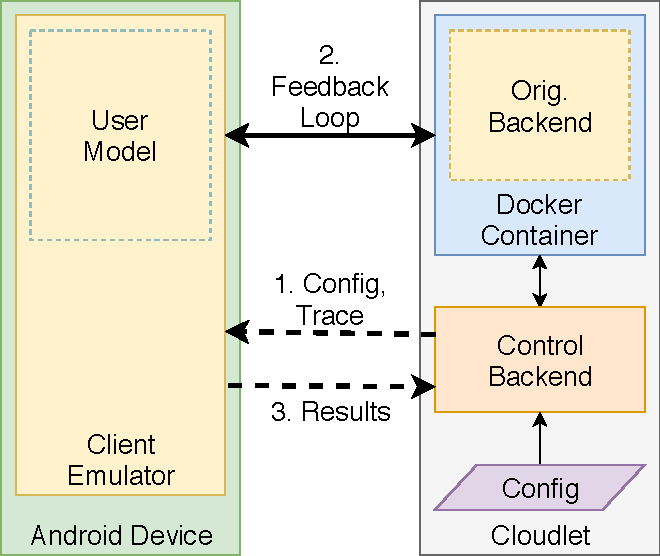
\includegraphics[width=.7\columnwidth]{publications/2019EdgeDroid/img/TraceReplay_GenArch}
    \caption{Architecture of the benchmarking suite.}\label{paper:olguinmunoz2019edgedroid:fig:TraceReplayArch}
\end{figure}

%In the following, we will detail the implementation of EdgeDroid 1.0.

The system architecture is composed of a \emph{cloudlet}, where one or more instances of the target application run, and one or more client devices, as pictured in \cref{paper:olguinmunoz2019edgedroid:fig:TraceReplayArch}.
These correspond to completely unaltered instances of the target application, running inside containers~\cite{docker}.
This allows the suite to extract metrics from them while remaining transparent to the application.
Here we also deploy the central component of EdgeDroid 1.0, the \emph{control backend}.

The \emph{control backend} is implemented in Python 3.6.
Its main purpose is to act as a central point of control and configuration of the experiments, as well as to aggregate results.
It controls the execution of the \emph{application instances} and configures the experiment and client devices, while also collecting system metrics during the execution of the benchmarks.
The experiments are configured in a centralized manner to simplify scaling.
Backend and clients communicate over TCP, using a simple application-layer protocol which allows for remote configuration, transmission of the trace data and result data, and synchronization of clocks across the system.
Note that although in the current implementation of the system the backend runs co-located with the \emph{application instances} on the cloudlet, we plan on implementing functionality for distributed monitoring from a separate computer and/or across multiple cloudlets.

The \emph{client emulators} correspond to Android applications with the main purpose of emulating a real user utilizing the target cognitive assistance application.
The emulators achieve this by mimicking the operation of real clients, but instead of obtaining the input data from the on-board sensors, they extract it from the previously recorded trace.
They replay this data over the network to the \emph{application instances} employing, as mentioned in \cref{paper:olguinmunoz2019edgedroid:sec:background}, a \emph{user model}, while simultaneously collecting client-side statistics and measurements.

The \emph{client emulators} are remote-controlled --- no interaction with a user is necessary once the application is initialized, simplifying large scale scenarios.

For our initial iteration of the EdgeDroid 1.0 benchmarking suite, we implement a preliminary user model, depicted in \cref{paper:olguinmunoz2019edgedroid:fig:usermodel}, to run on the \emph{client emulators}, designed with a linear task model in mind.
In EdgeDroid 1.0, our model is that of a user who is totally impervious to poor system performance, and suffers no annoyance, fatigue, frustration, nausea or other shortcomings of real human users.
This leads to a model of a user who responds in a precisely reproducible and deterministic manner to the same system stimulus every time.
In the future, we envision building upon this approach with many more human-like user models that more accurately emulate attributes such as fatigue and annoyance.

Each \emph{step} (i.e.\ segment) of the trace is played out to the backend until \emph{feedback} is received. If no feedback is received before the end of the step, it is replayed a pre-configured numbered of times before completely aborting the task (i.e.\ giving up).
Note that this model makes no distinction between positive and negative feedback, as both simply require the user to perform a specific action which is included in the trace.


\begin{figure}[tb]
    \centering
    \adjustbox{scale=0.7}{
    \ttfamily\centering%\fbox{%
    \begin{tikzpicture}[align=center,
        node distance=.5cm and 1.5cm,
        every initial by arrow/.style={-{Latex[length=2mm]}}]
        % Place nodes              
        \node [initial, state, minimum size=5em, initial text=] (play) {\textbf{Play}};
        \node [state, above right=of play, minimum size=5em] (change) {\textbf{Change}\\\textbf{step}};
        \node [state, below right=of play, minimum size=5em] (rewind) {\textbf{Rewind}};
        \node [state, accepting, above right=of rewind, minimum size=5em] (shutdown) {\textbf{Shut}\\\textbf{down}};

        % Draw edges
        \path[draw, -{Latex[length=2mm]}]
        (play) edge [out=270, in=180] node[below left] {Finished step but\\no feedback received} (rewind)
        edge [out=90, in=180] node[above left] {Received feedback} (change)
        edge [out=140, in=220,looseness=6] node[left] {Step\\not finished} (play)

        (change) edge [bend left=5] node[below right] {Step changed} (play)
        edge [out=0, in=90] node[above right] {All steps\\finished} (shutdown)

        (rewind) edge [bend right=5] node[above right] {Rewound} (play)
        edge [out=0, in=270] node[below right] {Too many\\rewinds} (shutdown);

    \end{tikzpicture}
}%}
    \captionof{figure}{Preliminary user model.}\label{paper:olguinmunoz2019edgedroid:fig:usermodel}
\end{figure}

\section{Use Cases}\label{paper:olguinmunoz2019edgedroid:sec:usecases}

\begin{table}[tb]
    \centering%
    \small%\ttfamily%
    \caption{Hardware used in the experiments.}%
    \label{paper:olguinmunoz2019edgedroid:tbl:cloudletclienthardware}%
    \begin{tabular}{@{}l@{\qquad}lclcl@{}}
        \toprule
         & \textbf{CPU}
         & \makecell{\textbf{Freq.}\\\textbf{[\si{\giga\hertz}]}}
         & \textbf{Cores}
         & \makecell[c]{\textbf{RAM}\\\textbf{[\si{\giga\byte}]}}
         & \makecell{\textbf{Operating}\\\textbf{System}}                                               \\
        \midrule
        \textbf{Cloudlet}
         & \makecell[bl]{Intel{\textregistered}\ Core{\texttrademark}\\i7--6700}
         & 3.4
         & 4
         & 32
         & \makecell[bl]{Ubuntu 17.10,\\kernel v4.13.0}                             \\
        \textbf{Clients}
         & \makecell[bl]{ARM{\textregistered}\\Cortex{\texttrademark}--A53}
         & 1.3
         & 4
         & 2
         & Android 7.0                                                             \\
        \bottomrule
    \end{tabular}%
\end{table}


In this section, we demonstrate the practical utility of EdgeDroid 1.0 through scalability measurements of real cognitive assistance application running on a cloudlet.
The questions we aim to answer relate to the ability of EdgeDroid 1.0 to provide relevant and accurate metrics on the performance of human-in-the-loop applications running on edge computing infrastructure.

Of particular interest is the ability to provide information about scaling limits in terms of latencies at both micro and macro levels.
We envision for instance a system designer performing the set of experiments detailed in this section.
The presented results would allow them to identify a bottleneck in performance.
From that they could extrapolate to how they need to scale their system hardware to manage their expected load, or they might conclude that their wireless link is not good enough for the average case.
They can also obtain real-time measurements to determine runtime measures to optimize performance, such as load balancing.
On the other hand, imagine an application developer who wishes to optimize their application.
EdgeDroid 1.0 would allow them to extract valuable information on where to focus their efforts.

%\todo[inline]{Also keep in mind that a perhaps more important question relates to on-line application optimization. Think about measures that can be applied at run-time on the side of the infrastructure to improve application performance - this is what one would like to explore here in this section.}

We chose the open source \emph{Gabriel} platform~\cite{ha2014towards} running the LEGO assistance application~\cite{chen2017empirical} for our experimentation.
This application guides a user through the assembly of a 2-dimensional LEGO model with visual and auditory instructions.
This functionality can be observed online.\footnote{\url{https://www.youtube.com/watch?v=7L9U-n29abg}}
We chose it due to its maturity and stability compared to other applications which run on the \emph{Gabriel} platform, as well as the relative simplicity of the task it performs.
The application employs a straightforward, linear task model as the one described in \cref{paper:olguinmunoz2019edgedroid:sec:background}.
Each state only allows for one specific correct action by the user, and any other action triggers negative feedback until the application is reset to the previous state.
The application has several different LEGO models to choose from, all of them roughly equal in complexity.
The specific task chosen for the experiments detailed in this section consists of the assembly of a 7-piece LEGO model.
The task has 7 distinct steps, and takes an average of approximately 2 minutes for a normal, untrained user to perform.
The input to the task model consist of a video stream captured either by an Android phone or a Google Glass wearable.

It should be noted that the \emph{Gabriel} platform by design always sends an acknowledgment for each input it receives, even when it is discarded, allowing us to measure latency for all inputs.


\cref{paper:olguinmunoz2019edgedroid:tbl:cloudletclienthardware} shows the hardware and software specifications for the cloudlet and the clients.
The components communicated through a single consumer-grade WiFi (IEEE 802.11n, \SI{2.4}{\giga\hertz}) access point.
We considered exclusively off-the-shelves hardware and software.
To minimize interference during the measurements, we locked the wireless link to the least congested available channel.
%Intel\textregistered \@ TurboBoost\texttrademark \@ technology was activated on the cloudlet CPU and the frequency of all cores locked to \SI{3.7}{\giga\hertz} to ensure consistency across experiments.

To ensure statistical independence between each emulated user, the initialization of each client emulator was subject to a random delay within a predefined window of time at the beginning of each run.
This way, the time between the start of any two clients in any repetition of the experiment is stochastic, leading to independent samples from each.
We also only take into account metrics collected while \emph{all} clients were concurrently running.

Our measurements were obtained from series of scenarios, repeated 100 times each.
We performed three \emph{optimal} scenarios with 1, 5 and 10 clients each, the signal strength of the WiFi link being an excellent \SI{-40}{\dBm}.
Next, a scenario where the 10 clients were moved to another room roughly \SI{10}{\meter} away, thus degrading the network link to an average measured strength of \SI{-73}{\dBm}.
Finally, we studied an additional optimal single-client scenario focused on latency distributions and jitters within application execution path.
This scenario is used to showcase the utility of EdgeDroid 1.0 for application developers.

\section{Results}\label{paper:olguinmunoz2019edgedroid:sec:results}

\begin{figure}
    \centering%
    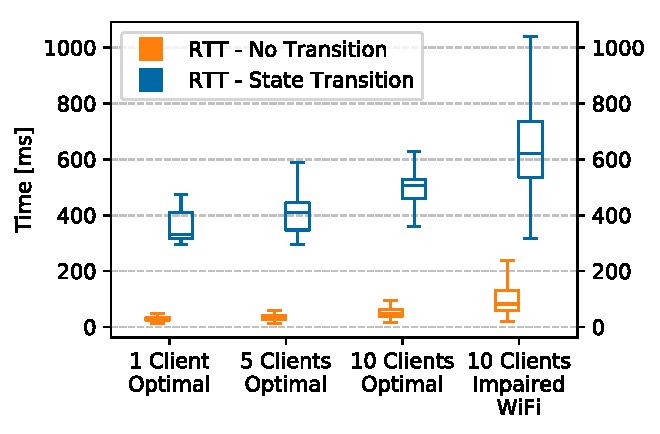
\includegraphics[width=.85\columnwidth]{publications/2019EdgeDroid/plots/comparison/nofonts/rtt_fb_vs_nofb}%
    \caption{Comparison of round-trip-times for inputs that triggered a state transition in the task model versus inputs that did not.}%
    \label{paper:olguinmunoz2019edgedroid:fig:comparison:rtt}%
\end{figure}%
\begin{figure}
    \centering%
    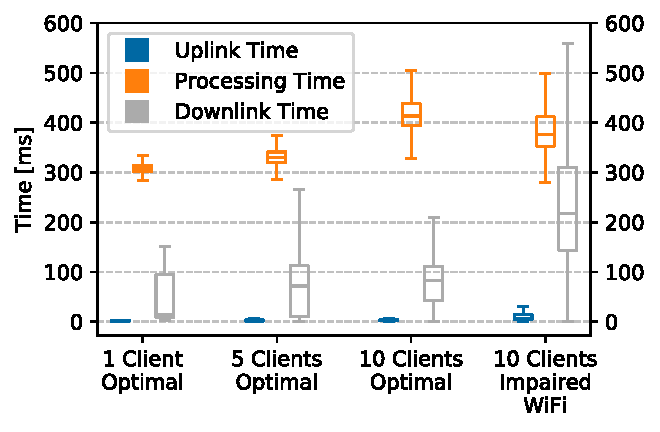
\includegraphics[width=.85\columnwidth]{publications/2019EdgeDroid/plots/comparison/nofonts/box_feedback}%
    \caption{Distribution of latency across system components for inputs that triggered a state transition in the task model.}%
    \label{paper:olguinmunoz2019edgedroid:fig:comparison:feedback}%
\end{figure}%
\begin{figure}%
    \centering%
    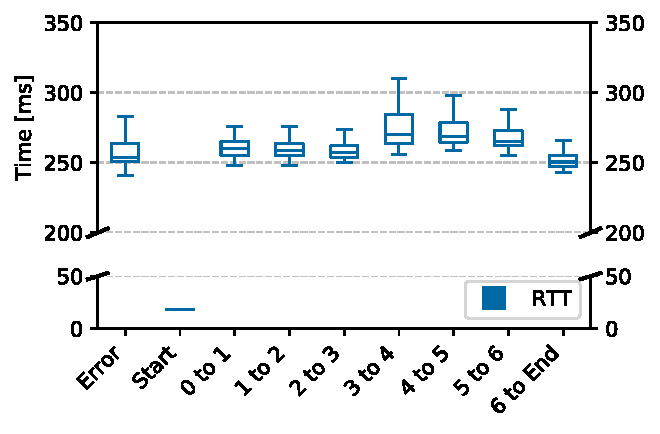
\includegraphics[width=.85\columnwidth]{publications/2019EdgeDroid/plots/comparison/nofonts/box_taskstep}%
    \caption{Round-trip-times for input-feedback cycles associated with state transitions in the internal task model for a single client connected over an optimal wireless link.}%
    \label{paper:olguinmunoz2019edgedroid:fig:comparison:tasksteps}
\end{figure}%

%In \cref{fig:comparison:feedback,fig:comparison:rtt,fig:comparison:tasksteps} we show some of the results obtained from the use case scenarios.
The results presented in this section provide valuable insights on both the system limits as well as on the application itself.

\cref{paper:olguinmunoz2019edgedroid:fig:comparison:rtt} presents a comparison of the total measured round-trip-times (RTTs) both for inputs which caused a state transition and inputs that did not.
Next, \cref{paper:olguinmunoz2019edgedroid:fig:comparison:feedback} shows a comparison of the distribution of latencies across system components for inputs that caused an internal state change in the task model of the application.
We differentiate according to the three main components contributing to latency, namely \emph{uplink} and \emph{downlink transmissions}, and \emph{backend processing}.
Finally, \cref{paper:olguinmunoz2019edgedroid:fig:comparison:tasksteps} depicts the distribution of RTTs for each transition in the internal task model for a single client connected over an optimal wireless link.
These metrics were calculated by recording the measured input-feedback cycle delay corresponding to a change in state within the application.
Thus, for instance, the measurements located at column ``3 to 4'' in the figure correspond to the aggregated round-trip-times for every input-feedback cycle corresponding to a change from state 3 to state 4 within the application task model, for the 100 repetitions of the scenario.

In the following discussion we will refer to inputs which triggered a transition in the task model as \emph{feedback-rich inputs} and those that did not as \emph{feedback-less inputs}.

For the analysis of these results, we will take into consideration the bound of \SI{600}{\milli\second} response time for step-by-step task-guidance derived by the authors of~\cite{chen2017empirical}.
This bound marks the point after which further delays in the delivery of feedback to the user start to negatively affect user experience, and allows for a straightforward evaluation of the responsiveness of the system.

We will begin our analysis of the experiment results with \cref{paper:olguinmunoz2019edgedroid:fig:comparison:rtt}.
These results present a stark contrast in the round-trip-times for inputs which cause a state transition versus inputs that do not, with RTTs for the former being up to an order of magnitude greater.
It's worth mentioning though that responses to feedback-less inputs are invisible to the user, and are just included here as a sort of baseline to compare feedback-rich round-trip times with.

We can identify a pair of interesting effects in the scaling of the task-guidance \gls{WCA} application.
One, scaling behavior for the application seems to be linear with respect to the number of clients.
Two, in the case of the impaired WiFi, the effect on the feedback-rich inputs is very pronounced, with the average of the RTTs for these inputs being over the previously discussed bound of \SI{600}{\milli\second}.

It is worth noting that already at just 10 clients the response times for feedback-rich inputs are very close to the bound.
Looking at this through the lens of a an application developer, it could hint at a need for optimization of the later parts of the application pipeline, since RTTs for inputs which are discarded in the detection stage of the pipeline (i.e.\ feedback-less inputs) are still well below \SI{200}{\milli\second}.

EdgeDroid 1.0 allows researchers to zoom into specific components of the application feedback loop, as exemplified by \cref{paper:olguinmunoz2019edgedroid:fig:comparison:feedback}.
From this figure it is clear that the main component which contributes to latency in the optimal case is the backend processing, further lending credibility to our previous comment on the need for optimization.
Nevertheless, when the link quality decreases, the delays on the downlink start to overshadow the delays on the processing.
Here, the downlink time sometimes almost reaches the ideal bound by itself.
A system designer might then conclude from this that in order to be able to scale the application, their focus needs to be on improving the quality of the wireless link before increasing the processing power on the backend.

Finally, EdgeDroid 1.0 allows even more insights to be gained by homing in to individual steps in a task-guidance \gls{WCA}. Consider \cref{paper:olguinmunoz2019edgedroid:fig:comparison:tasksteps}.
The figure shows clears spikes in latencies at the transitions from task state 3 to 4 and from task state 4 to 5, which could indicate to the application developer that these specific transitions are ripe for optimization.

\section{Conclusions \& Future Work}\label{paper:olguinmunoz2019edgedroid:sec:conclusions}

Benchmarking human-in-the-loop applications is hard, given their tight interaction with human users who complicate the scaling and repeatability of experiments.
In this paper, we have presented a benchmarking suite for this type of applications, called EdgeDroid 1.0, capable of cutting out the need for users in performance evaluations.
We achieve this by employing pre-recorded sensory input traces which we play over the network to the real application backend, employing a parameterized user model to react to feedback.
We demonstrate its utility through a series of use case scenarios, from which we are able to extract metrics regarding latency both in regards to the application itself and the hardware stack.
We believe the EdgeDroid 1.0 suite thus represents an important first step towards enabling inexpensive and low-complexity large-scale research on the scaling limits of this type of applications, a requirement for wide adoption of the technology.

Nonetheless, there is still future work to be done.

The user model presented in this paper is only preliminary, and we are currently conducting research in characterizing user behavior when interacting with \gls{WCA} applications in order to present a more complete model in the future.
As mentioned in \cref{paper:olguinmunoz2019edgedroid:sec:implementation}, in EdgeDroid 1.0, our model is that of a user who does not suffer any of the shortcomings of real human users such as annoyance, fatigue, frustration, nausea.
Rather, EdgeDroid 1.0 models a perfectly stoic user who is like an automaton and responds in a precisely reproducible and deterministic manner to the same system stimulus every time.
Of course, no real human user is an automaton.
In the future, we envision creating  many versions of EdgeDroid (i.e., EdgeDroid 2.0, EdgeDroid 3.0, etc.) that embody more human-like user models that more accurately emulate attributes such as those mentioned above.
Experimental validation of these human-like user models via user studies will be an important part of our future work.

We are also working on expanding the benchmarking suite to also work first with other types of Wearable Cognitive Assistance, and later with other categories of human-in-the-loop applications.
Other types of \glspl{WCA} we will consider in future iterations of the tool include real-time task-assistance \gls{WCA} applications (such as the Ping-Pong application described in~\cite{chen2017empirical}), which don't have a linear task model like task-guidance \gls{WCA} and have tighter latency bounds and context- and information-providing \gls{WCA} applications, for instance, applications which recognize faces and provide relevant social-media information related to that person.
The latter also do not have a linear task model, but present more lax latency bounds.

\begin{acks}
    We thank Bobby Klatzky and Dan Siewiorek for many valuable technical discussions relating to this research.
    We also thank our shepherd, Wenjun Hu, and the anonymous reviewers for helping us improve the paper.
    This research was supported in part by the \gls{NSF}, grant number \verb|CNS-1518865|, the VINNOVA grant \verb|MERIT (2017--05232)|.
    Additional support was provided by Intel,\ Vodafone,\ Deutsche~Telekom,\ Verizon,\ Crown~Castle,\ NTT,\ and the Conklin~Kistler family fund.
    Opinions, findings, conclusions or recommendations expressed in this material are those of the authors and do not necessarily reflect the view(s) of their employers or the mentioned funding sources.
\end{acks}
